\documentclass[a4paper]{report}

\usepackage[greek, english]{babel}
\usepackage[utf8]{inputenc}
\usepackage{amsmath}
\usepackage{graphicx}
\usepackage[colorinlistoftodos]{todonotes}
\usepackage{tikz}
\usetikzlibrary{shapes,arrows}
\usepackage{verbatim}
\usepackage{listings}


\newcommand{\inlinecode}{\texttt}
\renewcommand{\thesection}{\arabic{section}}

\title{psax Design Report}

\author{Will Oursler}

\date{\today}

\begin{document}
\maketitle

\section{Overview}

The system described herein extends UNIX systems to implement ``search folders'': curated directories created from queries for contents and file attributes. While users typically create directories based on shared attributes of files in them, current file-systems do not allow for definition of directories based on these attributes. Extending the UNIX file-system to support this model of use will make it more powerful and intuitive.

I propose responsive but efficient daemon (loosely modeled after the popular UNIX tool \inlinecode{cron}). It is assumed that search folders lagging a few minutes behind the system in day to day usage is acceptable but if a user mounts a new search folder then it must immediately be available for use once the process used to initialize it terminates.

In the spirit of \inlinecode{cron}'s name being derived from \textgreek{χρόνος} for time, \inlinecode{psax} is derived from \textgreek{f'aximo}, greek for search or investigation.

\section{Usage Example}

A photographer wants to create a folder of all her recent pictures (e.g. pictures taken in the last 3 days). She runs the command

\begin{center}
\inlinecode{searchmount "\textasciitilde/Recent Pictures" \textasciitilde/Pictures -mtime -3}
\end{center}

The mounted folder will always contain symlinks of the pictures from the last 3-4 days (the extra day is because \inlinecode{psax} will only recheck files it has confirmed match the query about once a day). If at any later date she puts a new batch of pictures in any subdirectory of \inlinecode{ \textasciitilde/Pictures } then symlinks will appear within a few minutes.

\section{Design Description}

\begin{figure}[h!]
  \centering
  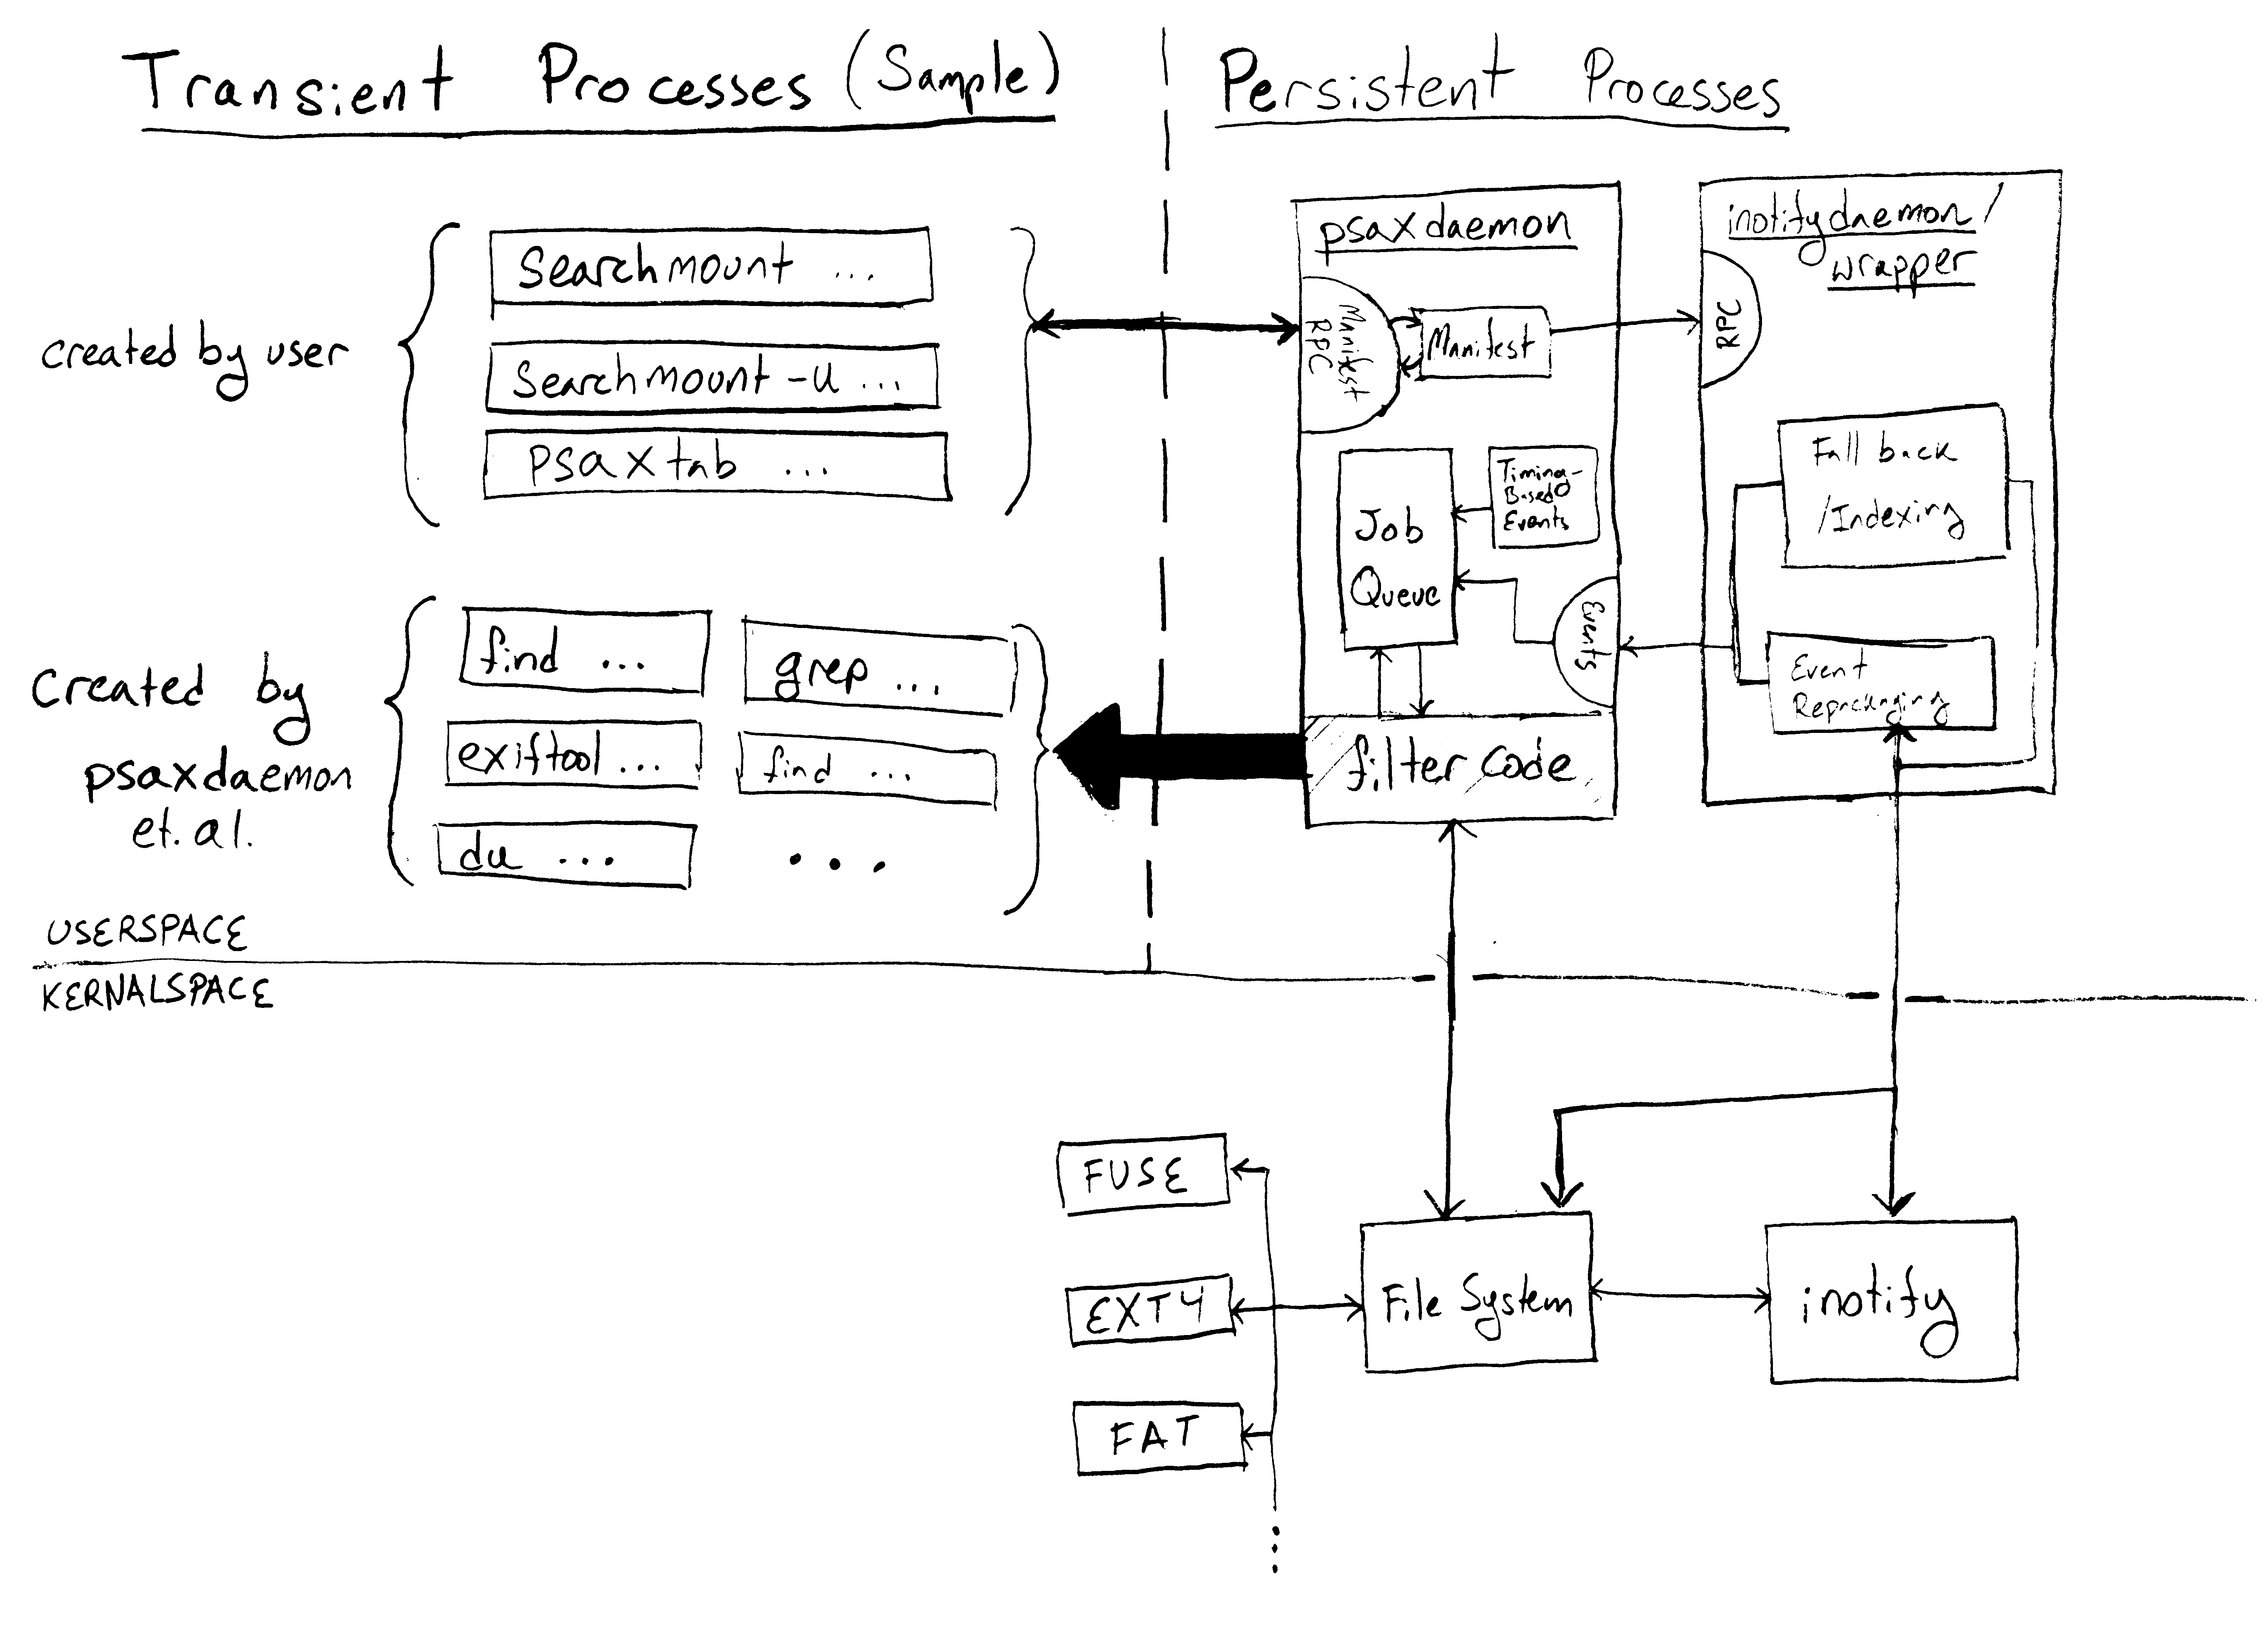
\includegraphics[width=1.0\textwidth]{structure}
  \caption{A rough overview of the modules involved in \inlinecode{psax} and their interconnections. Notice that the processes that the user interacts with (\inlinecode{searchmount}, \inlinecode{psaxtab}) are wrappers on a \inlinecode{psaxdaemon} RPC.}
\end{figure}

Figure 1 (on the next page) displays the overall structure of the system. Its various parts and interfaces are described below.

\subsection{Requirements and Overhead}

\inlinecode{psax} is designed to run in userspace with minimal kernel modification\footnote{\inlinecode{psax} uses \inlinecode{FUSE} -- Filesystem in Userspace -- to avoid modifying kernel code. FUSE is prepackaged in many package repositories, so it not an onerous requirement.}. Each user is responsible for maintaining their own table of descriptions of search folders (a \inlinecode{psaxtab}). A userspace daemon (the \inlinecode{psaxdaemon}) is responsible for ensuring that these descriptions are properly mounted and maintained.

\subsection{Daemon RPC and Search Folder Construction}

The \inlinecode{psaxdaemon} defines an RPC that allows it to interact with a manifest of search folders. Each entry in this manifest includes the path to the search folder, a list of paths to the searched directories, and a context used to select and modify filters.

For brevity, the exact form of this RPC is left to the implementer.

When a new entry is added to the manifest, an \inlinecode{inotify} watch is added through the daemon, and a ton of jobs are added to the job queue, as the search is run for the first time.

\subsection{Storing Results}

\begin{figure}[h!]
  \centering
  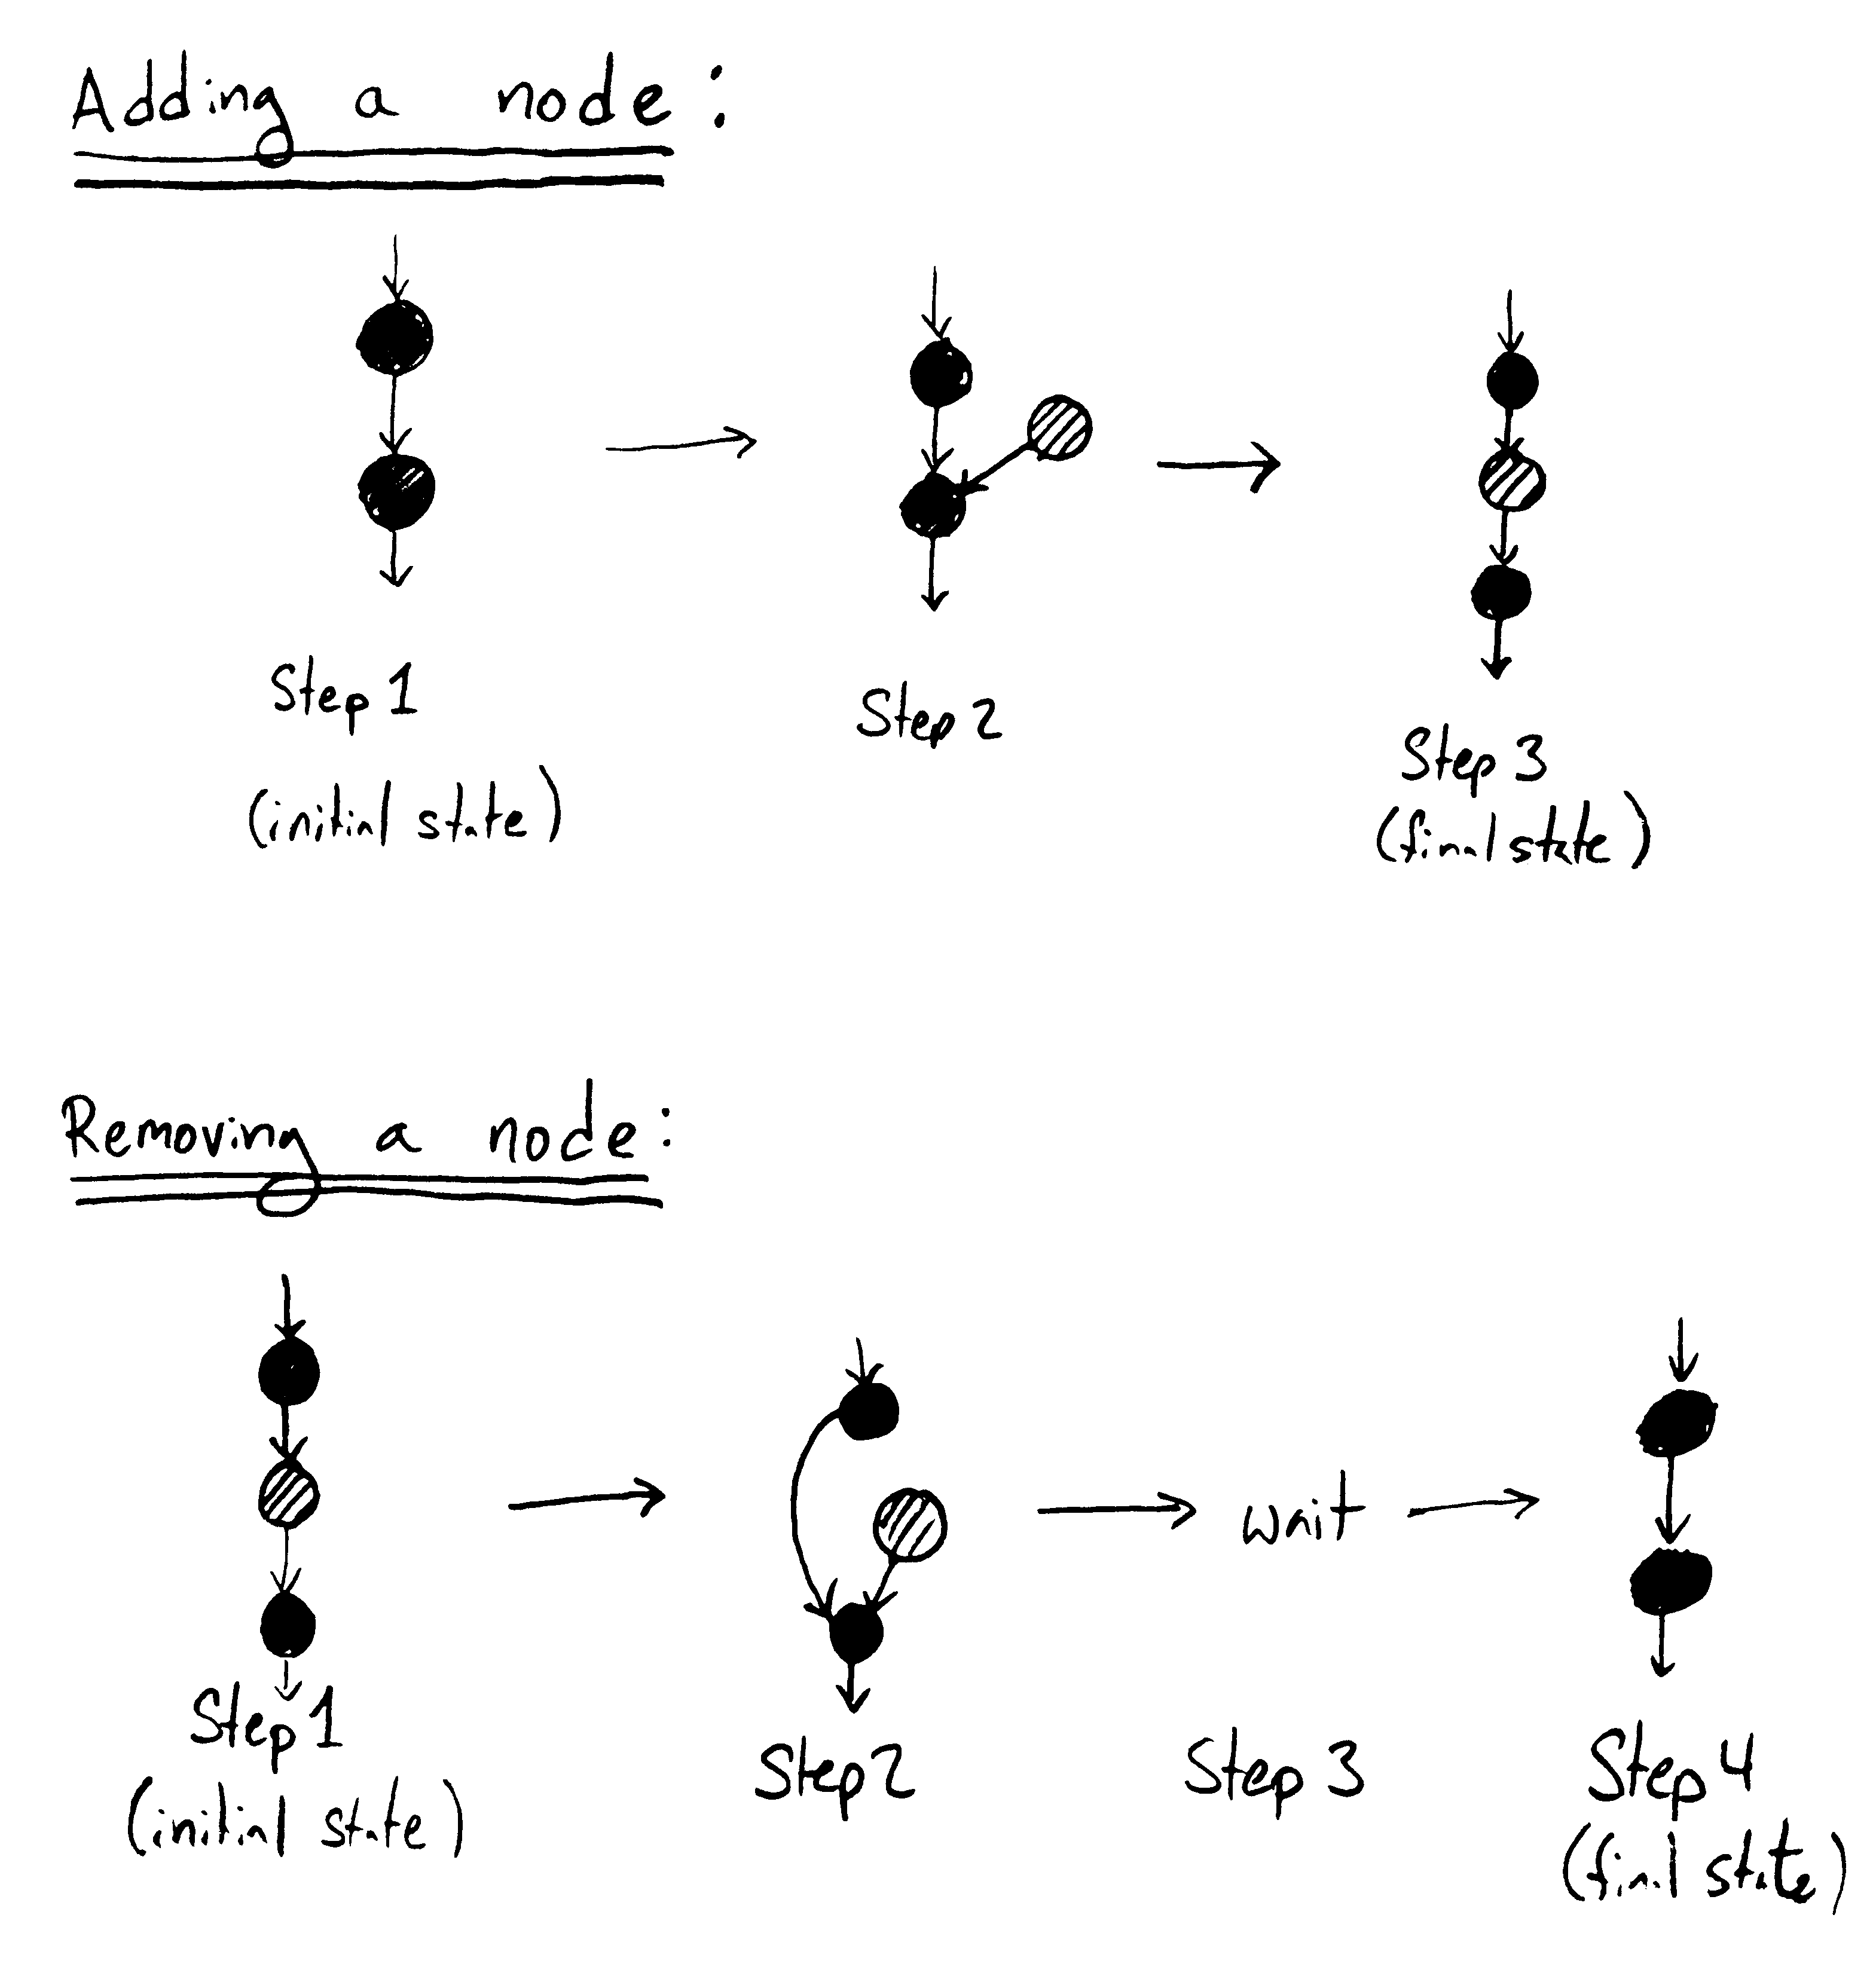
\includegraphics[width=0.5\textwidth]{addrm}
  \caption{The process for adding and removing elements in a linked list so that existing references produce sensible results so long as they were acquired recently. The element being added or removed is shown half-shaded.}
\end{figure}

Because our searches are expensive, \inlinecode{psaxdaemon} saves the results in a linked list in persistent databases on disk. Further details on the implementation of the linked list structure can be found in the following sections.

As detailed in Figure 2, of particular note is the delay inserted when removing a node. This delay should be implemented such that it does not hang up general execution - a separate thread is appropriate. A delay of around $0.5$ seconds should be generous without being onerous.

\subsection{Presenting results with \inlinecode{FUSE}}

\inlinecode{psax} presents cached search results to the user. These cached results are stored as a linked list in one of the provided key-value stores. There are two such key-value stores involved in this process.

\begin{description}
\item[\inlinecode{first\_entry.db}] Contains a mapping from the \inlinecode{dirname} of the mounted directory to a \inlinecode{DirEntryPointer} for the first entry of that directory.
\item[\inlinecode{next\_entry.db}] Contains a mapping from \inlinecode{DirEntryPointer} to \inlinecode{DirEntryPointer}. Enforced to be acyclic, and operations on this list are carefully designed to be atomic, such that FUSE requests can be fulfilled at any time.
\end{description}

\inlinecode{DirEntryPointer}s are objects of \inlinecode{(filename, folder\_id)}, where \inlinecode{filename} is the full path to a file of interest and \inlinecode{folder\_id} is used to ensure that the same file can appear in multiple search folders. They are serialized to strings with \inlinecode{JSON}.

To support a FUSE-like system\footnote{In reality, this API is a sort of silly wrapper to place around FUSE, but I'll humor the provided spec and follow it exactly.} the following API is implemented.

\begin{description}
\item[\inlinecode{DirEntryPointer get\_first\_directory\_entry(String dirname)}]

Perform the lookup in \inlinecode{first\_entry.db}.

\item[\inlinecode{DirEntryPointer read\_next\_directory\_entry(DirEntryPointer previousFile)}]

Simply perform the lookup in \inlinecode{next\_entry.db}. If \inlinecode{previousFile} produces an invalid key, then the \inlinecode{DirEntryPointer} is invalid, and \inlinecode{NULL} should be returned. Any given \inlinecode{DirEntryPointer} is only guaranteed to remain valid for a few seconds.

\item[\inlinecode{String file\_name( DirEntryPointer entry )}]

Returns a modified version of the string \inlinecode{entry.filename}.

Maps \inlinecode{"/path/to/dir/name.ending"} to \inlinecode{"search\_dir/name$(n)$.ending"}, where $n$ is the smallest number such that the name is unique. In the $n=0$ it can be omitted completely (i.e. the filename remains unchanged). Notice that under this scheme the naming of elements can depend on the order, so for best performance, the list should be kept in lexicographic order on \inlinecode{name.ending}.

\item[\inlinecode{String read\_symbolic\_link( DirEntryPointer entry )}]

This is trivial. Simply return \inlinecode{entry.filename}.

\end{description}

\subsection{\inlinecode{inotify} wrapper daemon}

To ensure that relevant new files are quickly discovered, \inlinecode{inotify} is used. When a new \inlinecode{searchmount} command is issued, directories of interest (and their subdirectories) are watched. inlinecode{psax} will implement a wrapper around inotify that will both handle the recursion and provide a seamless fallback for efficiency's sake.

\subsubsection{Maintaining directory structure}

When a directory is watched by the daemon, subdirectories must also be watched. Subsequently, the daemon must carefully react to changes in directory structure.

\subsubsection{Fallback}

If the number of \inlinecode{inotify} watches approaches \inlinecode{inotify.max\_user\_watches}, or if a directory is being updated with such frequency that updates are a performance concern, the daemon provides a fallback based on periodically checking the directory. At each check, it stores an index of paths to all files and \inlinecode{MD5} hashes of their content and metadata.

\subsubsection{RPC}

\begin{description}

\item[\inlinecode{void add\_watch( String dirname )}] Adds a watch. Once added, events resulting from changes in the given directory are queued with the \inlinecode{psaxdaemon}.

\item[\inlinecode{void rm\_watch( String dirname )}] Removes any existing watches on a directory, if they exists

\end{description}

\subsubsection{Events Provided to the \inlinecode{psaxdaemon}}

Each event logged by the inotify wrapper includes the following attributes:

\begin{description}
\item[base \inlinecode{dirpath}] Denotes which to full path of the watch this event is associated with. Single \inlinecode{inotify} changes may produce one event for each watch at most.
\item[sub \inlinecode{dirpath}] Denotes the path relative to the watch.
\item[event flag] Describes exactly what has happened. Valid event flags are:

\begin{description}
\item[\inlinecode{IN\_CREATE}] An heretofore unseen file has been created.
\item[\inlinecode{IN\_DELETE}] A previously relevant file has been deleted.
\item[\inlinecode{IN\_ATTRIB}] The meta-data of the file has been modified.
\item[\inlinecode{IN\_MODIFY}] The contents of the file have been modified.
\end{description}

\end{description}


Other \inlinecode{inotify} alerts are either ignored (i.e. \inlinecode{IN\_OPEN}/\inlinecode{IN\_CLOSE\_NOWRITE}) or remapped (i.e. \inlinecode{IN\_DELETE\_SELF} will be rephrased / deduplicated as a \inlinecode{IN\_DELETE}) as appropriate. A notable case is when files are moved. While it is sensible that renaming would create a \inlinecode{IN\_ATTRIB}, for consistency's sake it is best to create a pair of events (\inlinecode{IN\_CREATE} and \inlinecode{IN\_DELETE}).

\subsection{Filters}

While we initially want to support the same sorts of queries as GNU \inlinecode{find}, it is likely that we might want to issue other sorts of queries. We may wish to issue queries related to
\begin{itemize}
\item The content of ASCII encoded files. \inlinecode{find} does not include functionality for this, other utilities like \inlinecode{grep} do.
\item The times and locations in which photos were taken. These are often encoded in EXIF data included in files.
\end{itemize}

Filters support a wide array of different queries. Each filter takes a user-specified context as an argument. In the case of \inlinecode{find\_filter}, this context would be the set of flags the user would use with \inlinecode{find}.

\subsubsection{API / Filter Manifests}

Filters may be triggered over either files or directories when either content changes, meta-data changes, or both. These preferences are set with the following flags:

\begin{description}
\item[\inlinecode{WATCH\_DIRECTORIES\_ONLY}] This filter only acts upon the immediate contents of whole directories.
\item[\inlinecode{WATCH\_FILES\_ONLY}] This filter only acts upon files.
\item[\inlinecode{WATCH\_CONTENT}] Filter triggers when content changes.
\item[\inlinecode{WATCH\_METADATA}] Filter triggers when meta-data changes.
\end{description}

It's enforced that at least one of \inlinecode{WATCH\_CONTENT} or \inlinecode{WATCH\_METADATA} will be set \inlinecode{True} for every filter. Only one of \inlinecode{WATCH\_DIRECTORIES\_ONLY} and \inlinecode{WATCH\_FILES\_ONLY} may be set true.

\begin{description}
\item[\inlinecode{String[] apply\_to\_directory( String dirpath, String context )}] Runs over the directory and returns a list of all matching files. It is never called if \inlinecode{WATCH\_FILES\_ONLY} is set.
\item[\inlinecode{Boolean apply\_to\_file( String filepath, String context )}] Returns \inlinecode{true} if and only if the filter matches the file. It is never called if \inlinecode{WATCH\_DIRECTORIES\_ONLY} is set.
\item[\inlinecode{Number estimated\_cost( Number numbytes, Number numfiles)}] Returns an estimate, in seconds of the time required to process \inlinecode{numbytes} in \inlinecode{numfiles}. Strongly prefer a quick but rough estimate to an exact but slow one. This operation should be sufficiently inexpensive that it is not a timing consideration.
\end{description}

\subsection{Example: the \inlinecode{find} filter}

The find filter has \inlinecode{WATCH\_DIRECTORIES\_ONLY} and \inlinecode{WATCH\_METADATA} set \inlinecode{True}. It defines its  routines as follows:

\begin{description}
\item[\inlinecode{apply\_to\_directory}]

Each time this function is called, the command

\inlinecode{find $(dirname)$/* -maxdepth 0 $(context)$}

or an equivalent should be run. Note that this command does not act recursively as per spec. The resulting matches should be reformatted into a list and returned.

\item[\inlinecode{estimated\_cost}] This function should be fit with a linear regression over a range of reasonable real world trials.

\end{description}


\subsection{Job Queue}

Efficiency is a central concern. The \inlinecode{psaxdaemon} is susceptible to load spikes; moving or copying directories may create more work for \inlinecode{psax} than can be done immediately.

The daemon will maintain a queue of jobs, each with an associated estimated cost (calculated from the appropriate filter) and a time-to-live (TTL) counter. The counter should be set to roughly the number of short jobs it is acceptable to delay any given job by. It may be appropriate to have larger initial TTL counters for more expensive jobs.

The daemon will at each opportunity dequeue a job \emph{if and only if the total CPU usage of all currently running jobs is below a configuration parameter}. CPU Usage will therefore only modestly exceed this limit. Due to potential short term volatility in CPU usage, especially when a new process is starting, the daemon should wait a small amount of time between dequeuing jobs even if total CPU usage is low. For performance reasons, we may wish to increase this limit if overall CPU utilization is low, and vice versa.

\begin{figure}[h!]
  \centering
  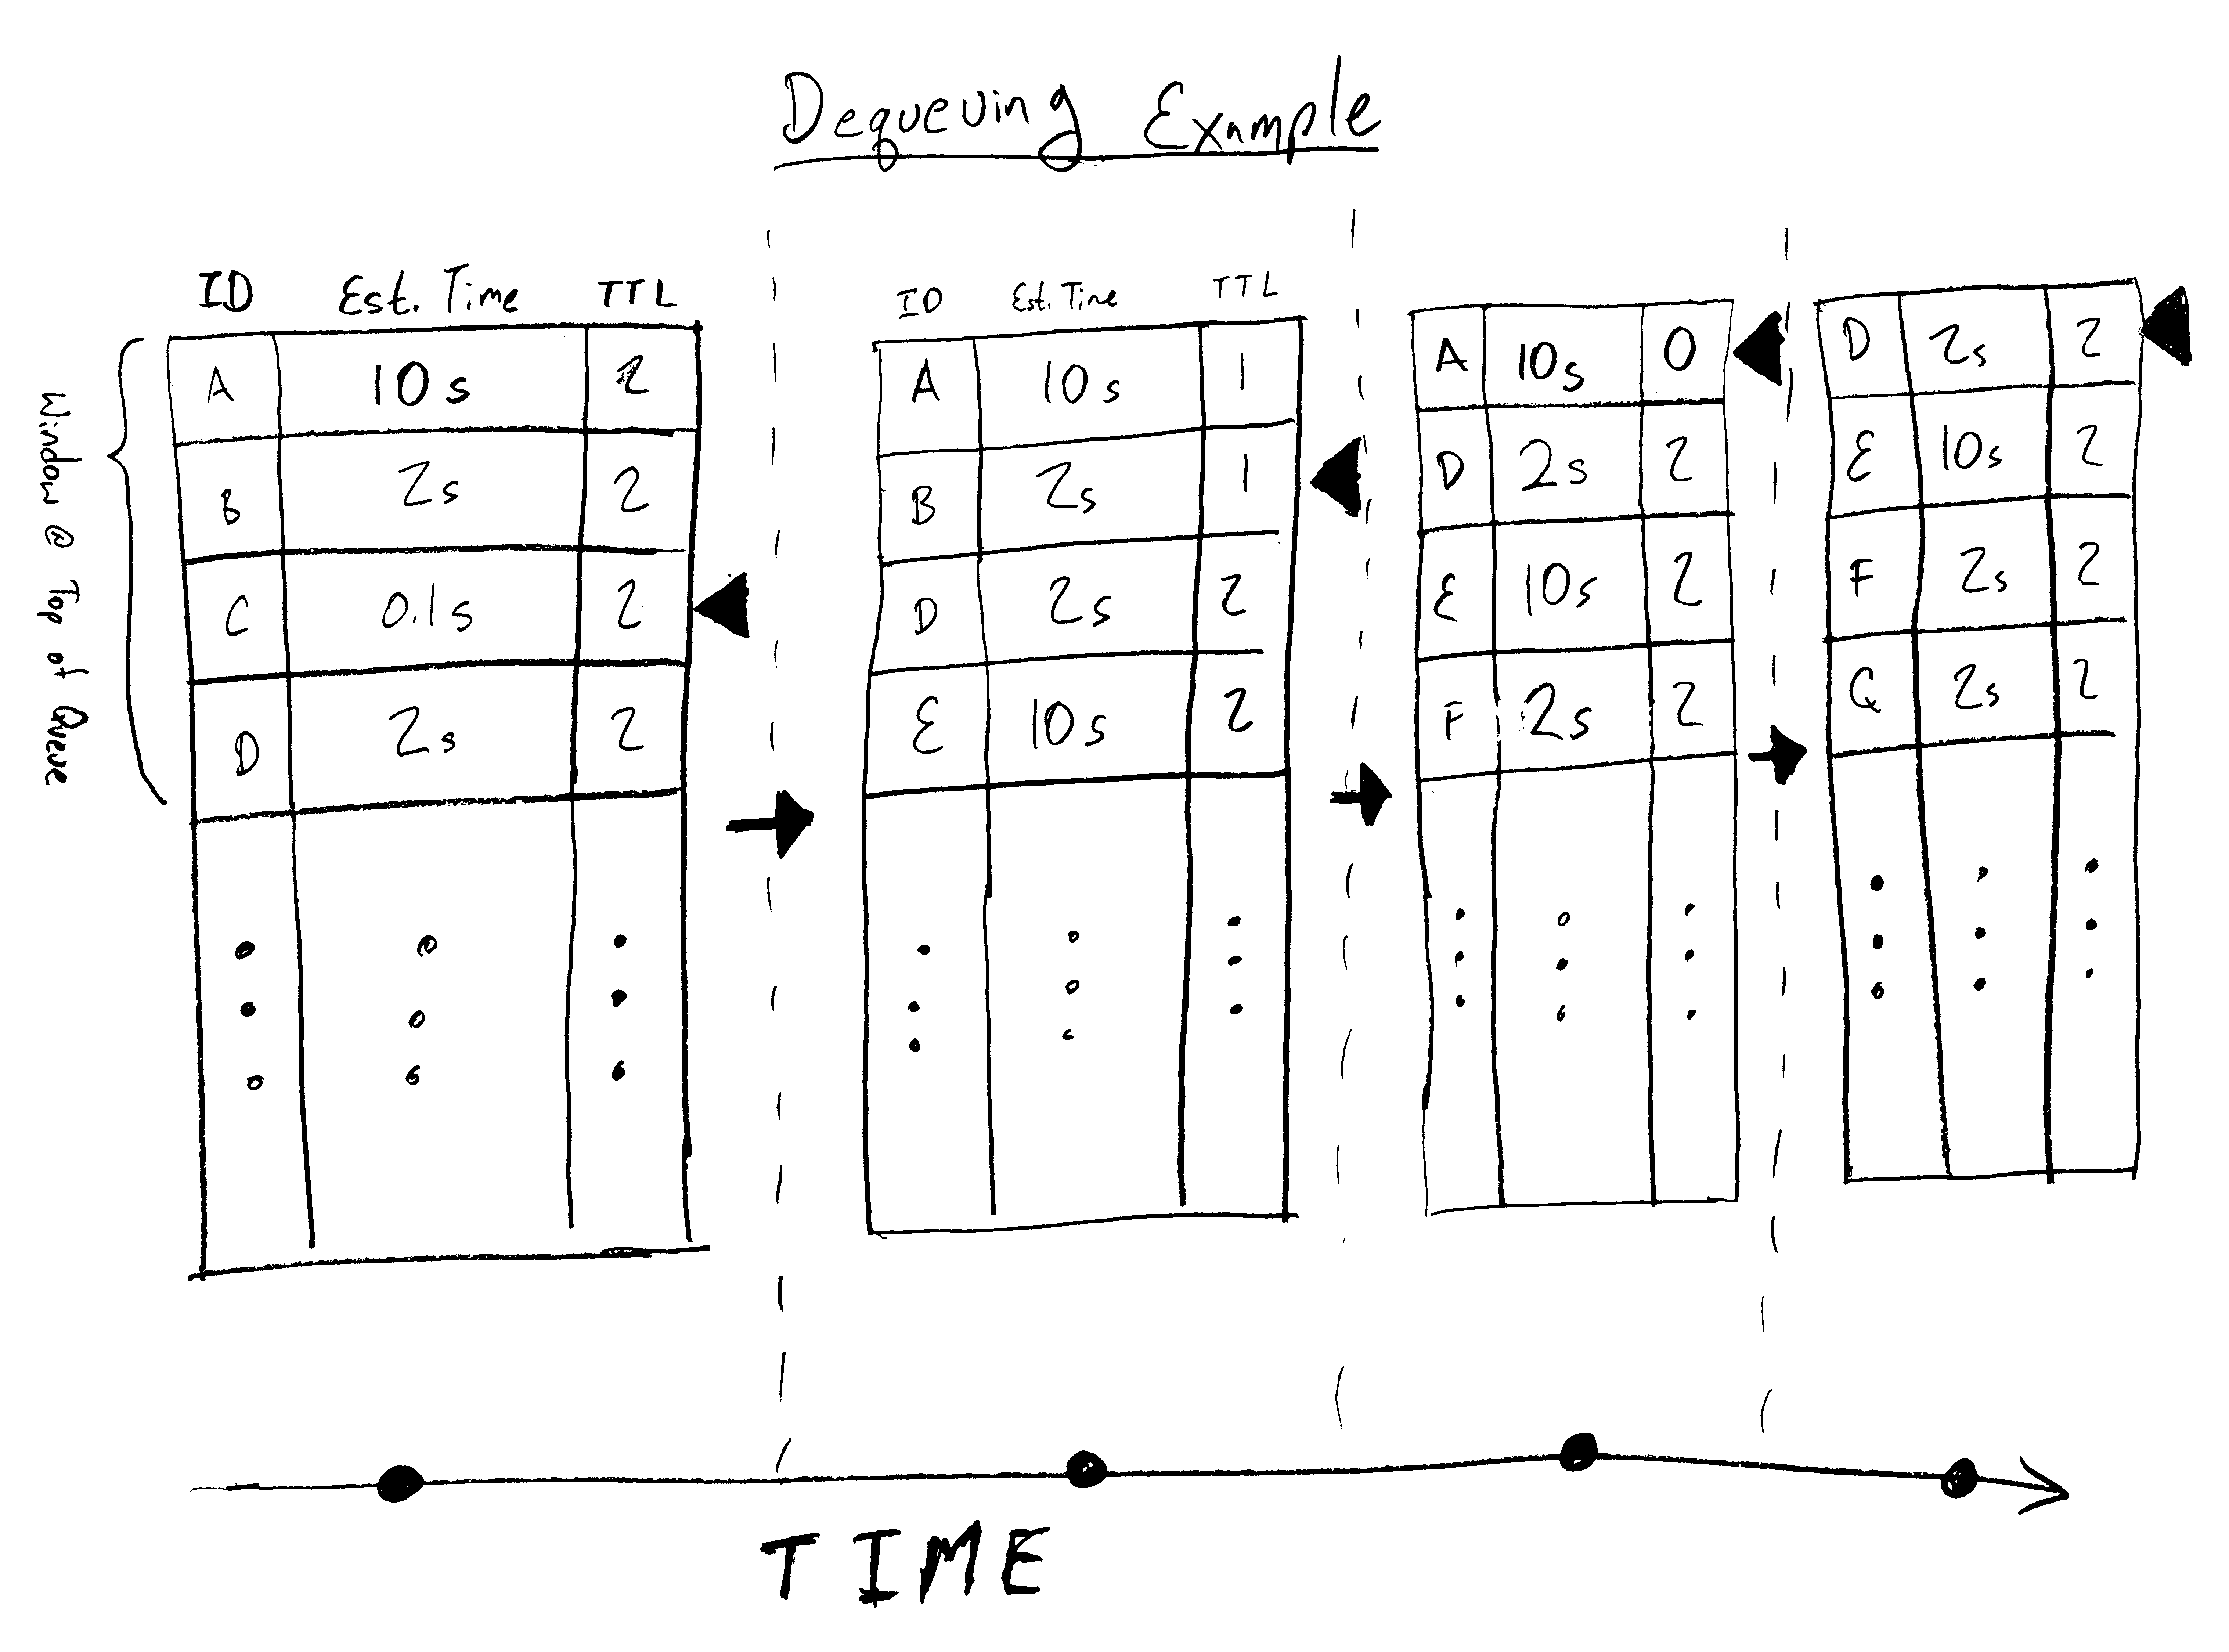
\includegraphics[width=1.0\textwidth]{dequeue}
  \caption{The dark triangles denote the element selected for dequeuing at every step. It is assumed that element $C$ is the only element in the list that takes less than $2s$.}
\end{figure}

\subsubsection{Dequeuing Algorithm}

We dequeue the first element of the queue with a TTL counter of $0$, or the smallest element (minimal TTL multiplied with expected time) if there is no element with TTL counter $0$. In the second case, if we select element $i$, then all $i$ members of the queue above the selected element have their TTL counters decremented.

The algorithm is demonstrated in Figure 3. Its performance characteristics are explored in the next section.

\section{Timing and Performance Analysis}

\subsection{GNU \inlinecode{find}}

Because find is used so integrally, timing analysis is appropriate. I propose running \inlinecode{find} in testing circumstances similar to those it will encounter under \inlinecode{psax} (specifically with \inlinecode{-maxdepth 0}).

I tried to create a quick script to get some order of magnitude estimates, but was unable to get good data with \inlinecode{time} - even for large numbers (around 1000) of 1MB files, total times as low as \inlinecode{0.000s} were reported on a standard Athena workstation (\inlinecode{BARKER-5-4}). This does not represent a good measurement because the process I used to create the test data (\inlinecode{dd}ing data from \inlinecode{/dev/urandom}) likely collocates data on disk in a rather unnatural way that \inlinecode{find} does well with.

\subsection{CPU Usage}

\inlinecode{psax} Explicitly keeps it's CPU Usage as low as possible while still completing jobs in a timely manner using the job queue. it includes a dynamically adjustable parameter that can be used to ensure good system performance at runtime.

\subsection{Dequeuing Algorithm}

As a baseline, we must ensure that any element on the queue will eventually be dequeued. We will first show that the first element must be dequeued in a finite number of operations, then extend the result to all elements.

If an element is at the front of the queue then at every step either it is either selected or an element below it is selected. In the first case, we are trivially done. In the second, the TTL counter of the first element will be decremented. Once this counter reaches $0$, the element will be selected immediately.

Once we know that the first element is removed in finitely many steps, we can ensure that any element will be dequeued by extension, since we know that within finitely many steps, it will move towards the top of the queue.

\subsection{Responses to Extreme Conditions and Further Improvements}

A number of situations have the potential to badly snare up a system like \inlinecode{psax}. These have served to motivate the design and are therefore a valuable reference during implementation.

\begin{description}

\item[Duplicated Work] \inlinecode{psax} explicitly does not redo work it has already done except on a predefined timetable.

\item[Freshness] There are no explicit freshness guarantees, and in fact \inlinecode{psax} may perform quite poorly in this respect if it is running on a machine with few resources to devote to it, as should perhaps be expected. At least one job is running at all times, however, so \inlinecode{psax} should always be working to ensure results are as fresh as available resources allow.

\item[Duplicated Filenames] As described, \inlinecode{psax} handles this problem by renaming files if and only if conflicts occur. Two files named $stuff.txt$ will be mapped to $stuff.txt$ and $stuff(1).txt$ in the search folder.

\item[Searching a \inlinecode{psax} Directory] Since \inlinecode{psax} is \inlinecode{FUSE}-based, this will work fine! One special case that must be handled, however, is that of a loop, where two search folders search each other. This must never be allowed to happen, but it is easy enough to avoid since internally \inlinecode{psax} associates non-recursive directories with every job.

\item[Persistence across restarts / crashes] Results of searches persist across downtime; \inlinecode{psax} doesn't even hiccup. If true persistence is required, the job queue, as well as any currently running jobs will need to be serialized and saved upon shutdown.

\end{description}

\section{Conclusion}

The above description of \inlinecode{psax} should be detailed enough to allow full implementation. What remains is primary fitting several parameters so that the system can perform well in a variety of real world situations.

\section{Acknowledgments}

Besides course staff, I worked with no one on this project.

\section{Word Count}

Around 2,600, including this word count, references, section titles and such. Hard to count with \LaTeX.

\section{References}

J. Saltzer  and  M. Kaashoek,  \textit{Principles  of  Computer  System  Design:  An  Introduction}.
Burlington,  MA:  Morgan  Kaufmann,  2

FUSE Project, \textit{fuse.sourceforge.net/}

inotify manual page, \textit{man7.org/linux/man-pages/man7/inotify.7.html}

\end{document}